% Options for packages loaded elsewhere
\PassOptionsToPackage{unicode}{hyperref}
\PassOptionsToPackage{hyphens}{url}
\PassOptionsToPackage{dvipsnames,svgnames,x11names}{xcolor}
%
\documentclass[
  12pt]{article}

\usepackage{amsmath,amssymb}
\usepackage{iftex}
\ifPDFTeX
  \usepackage[T1]{fontenc}
  \usepackage[utf8]{inputenc}
  \usepackage{textcomp} % provide euro and other symbols
\else % if luatex or xetex
  \usepackage{unicode-math}
  \defaultfontfeatures{Scale=MatchLowercase}
  \defaultfontfeatures[\rmfamily]{Ligatures=TeX,Scale=1}
\fi
\usepackage{lmodern}
\ifPDFTeX\else  
    % xetex/luatex font selection
\fi
% Use upquote if available, for straight quotes in verbatim environments
\IfFileExists{upquote.sty}{\usepackage{upquote}}{}
\IfFileExists{microtype.sty}{% use microtype if available
  \usepackage[]{microtype}
  \UseMicrotypeSet[protrusion]{basicmath} % disable protrusion for tt fonts
}{}
\makeatletter
\@ifundefined{KOMAClassName}{% if non-KOMA class
  \IfFileExists{parskip.sty}{%
    \usepackage{parskip}
  }{% else
    \setlength{\parindent}{0pt}
    \setlength{\parskip}{6pt plus 2pt minus 1pt}}
}{% if KOMA class
  \KOMAoptions{parskip=half}}
\makeatother
\usepackage{xcolor}
\setlength{\emergencystretch}{3em} % prevent overfull lines
\setcounter{secnumdepth}{5}
% Make \paragraph and \subparagraph free-standing
\makeatletter
\ifx\paragraph\undefined\else
  \let\oldparagraph\paragraph
  \renewcommand{\paragraph}{
    \@ifstar
      \xxxParagraphStar
      \xxxParagraphNoStar
  }
  \newcommand{\xxxParagraphStar}[1]{\oldparagraph*{#1}\mbox{}}
  \newcommand{\xxxParagraphNoStar}[1]{\oldparagraph{#1}\mbox{}}
\fi
\ifx\subparagraph\undefined\else
  \let\oldsubparagraph\subparagraph
  \renewcommand{\subparagraph}{
    \@ifstar
      \xxxSubParagraphStar
      \xxxSubParagraphNoStar
  }
  \newcommand{\xxxSubParagraphStar}[1]{\oldsubparagraph*{#1}\mbox{}}
  \newcommand{\xxxSubParagraphNoStar}[1]{\oldsubparagraph{#1}\mbox{}}
\fi
\makeatother


\providecommand{\tightlist}{%
  \setlength{\itemsep}{0pt}\setlength{\parskip}{0pt}}\usepackage{longtable,booktabs,array}
\usepackage{calc} % for calculating minipage widths
% Correct order of tables after \paragraph or \subparagraph
\usepackage{etoolbox}
\makeatletter
\patchcmd\longtable{\par}{\if@noskipsec\mbox{}\fi\par}{}{}
\makeatother
% Allow footnotes in longtable head/foot
\IfFileExists{footnotehyper.sty}{\usepackage{footnotehyper}}{\usepackage{footnote}}
\makesavenoteenv{longtable}
\usepackage{graphicx}
\makeatletter
\def\maxwidth{\ifdim\Gin@nat@width>\linewidth\linewidth\else\Gin@nat@width\fi}
\def\maxheight{\ifdim\Gin@nat@height>\textheight\textheight\else\Gin@nat@height\fi}
\makeatother
% Scale images if necessary, so that they will not overflow the page
% margins by default, and it is still possible to overwrite the defaults
% using explicit options in \includegraphics[width, height, ...]{}
\setkeys{Gin}{width=\maxwidth,height=\maxheight,keepaspectratio}
% Set default figure placement to htbp
\makeatletter
\def\fps@figure{htbp}
\makeatother

\addtolength{\oddsidemargin}{-.5in}%
\addtolength{\evensidemargin}{-1in}%
\addtolength{\textwidth}{1in}%
\addtolength{\textheight}{1.7in}%
\addtolength{\topmargin}{-1in}%
\makeatletter
\@ifpackageloaded{caption}{}{\usepackage{caption}}
\AtBeginDocument{%
\ifdefined\contentsname
  \renewcommand*\contentsname{Table of contents}
\else
  \newcommand\contentsname{Table of contents}
\fi
\ifdefined\listfigurename
  \renewcommand*\listfigurename{List of Figures}
\else
  \newcommand\listfigurename{List of Figures}
\fi
\ifdefined\listtablename
  \renewcommand*\listtablename{List of Tables}
\else
  \newcommand\listtablename{List of Tables}
\fi
\ifdefined\figurename
  \renewcommand*\figurename{Figure}
\else
  \newcommand\figurename{Figure}
\fi
\ifdefined\tablename
  \renewcommand*\tablename{Table}
\else
  \newcommand\tablename{Table}
\fi
}
\@ifpackageloaded{float}{}{\usepackage{float}}
\floatstyle{ruled}
\@ifundefined{c@chapter}{\newfloat{codelisting}{h}{lop}}{\newfloat{codelisting}{h}{lop}[chapter]}
\floatname{codelisting}{Listing}
\newcommand*\listoflistings{\listof{codelisting}{List of Listings}}
\makeatother
\makeatletter
\makeatother
\makeatletter
\@ifpackageloaded{caption}{}{\usepackage{caption}}
\@ifpackageloaded{subcaption}{}{\usepackage{subcaption}}
\makeatother

\ifLuaTeX
  \usepackage{selnolig}  % disable illegal ligatures
\fi
\usepackage[]{natbib}
\bibliographystyle{agsm}
\usepackage{bookmark}

\IfFileExists{xurl.sty}{\usepackage{xurl}}{} % add URL line breaks if available
\urlstyle{same} % disable monospaced font for URLs
\hypersetup{
  pdftitle={DOGE's Downsizing, Can AI Read the Reddit Room?},
  pdfauthor={Kevin Linares; Felix Baez-Santiago; Aria Lu; Gloria Zhou},
  pdfkeywords={Reddit, Federal Government, DOGE},
  colorlinks=true,
  linkcolor={blue},
  filecolor={Maroon},
  citecolor={Blue},
  urlcolor={Blue},
  pdfcreator={LaTeX via pandoc}}



\begin{document}


\def\spacingset#1{\renewcommand{\baselinestretch}%
{#1}\small\normalsize} \spacingset{1}


%%%%%%%%%%%%%%%%%%%%%%%%%%%%%%%%%%%%%%%%%%%%%%%%%%%%%%%%%%%%%%%%%%%%%%%%%%%%%%

\date{April 8, 2025}
\title{\bf DOGE's Downsizing, Can AI Read the Reddit Room?}
\author{
Kevin Linares\\
University of Maryland\\
and\\Felix Baez-Santiago\\
and\\Aria Lu\\
and\\Gloria Zhou\\
University of Michigan\\
}
\maketitle

\bigskip
\bigskip
\begin{abstract}
We investigate public sentiment on Reddit regarding the Department of
Government Efficiency's federal workforce reduction by classifying 400
labeled comments (28\% favor, 18\% neutral, 54\% oppose) using
supervised and unsupervised Large Language Models. Supervised models
showed moderate success, particularly with ``oppose'' comments, but
struggled with ``favor'' and ``neutral'' stances. Similarly, LLMs best
identified ``oppose'' sentiment but exhibited low precision for
``favor'' and ``neutral.'' These findings highlight the challenges of
accurately gauging nuanced public opinion on government policy changes
using automated methods on social media data.
\end{abstract}

\noindent%
{\it Keywords:} Reddit, Federal Government, DOGE
\vfill

\newpage
\spacingset{1.9} % DON'T change the spacing!


\section{Introduction}\label{sec-intro}

The newly formed Department of Government Efficiency (DOGE) has reduced
the federal workforce by almost 280,000 employees, a central pledge of
the current administration. This action has generated significant
apprehension among federal workers in regards to mental health and job
security. To understand the impact of DOGE's actions on federal worker
perceptions of job security, we labeled 400 Reddit comments on topics
related to the current reduction in \emph{federal} workforce by DOGE as
whether the author favored, opposed, or had a neutral stance. We use
these labels to build supervised learning models to predict stance.
Additionally, we employ unsupervised large language models (LLM) to
detect the stance of these Reddit comments from text, to further explore
appropriate models for this current topic.

\section{Methods}\label{sec-meth}

\emph{Data}. We collected Reddit comments from subreddits related to the
topic of interest in early March of 2024. This resulted in 12,553
comments which we preprocessed by removing web-URLs, replace special
characters (i.e., replaced ``@'' with ``at''), replaced numeric values
with their spelling, and confirmed the absence of duplicate comments. We
then randomly selected 400 comments (without replacement) and assigned
them to four graduate students for coding, categorizing each comment as
favoring, opposing, or neutral towards DOGE's approach to federal
workforce reductions. Table 1 presents the breakdown in percent of our
the comments we labelled and later use to train and evaluate our machine
learning models. A review of the comments revealed more negative
opinionated statements and reactions.

\begin{longtable}[]{@{}lr@{}}
\caption{Distribution of labeled Reddit comment data.}\tabularnewline
\toprule\noalign{}
outcome & Percent \\
\midrule\noalign{}
\endfirsthead
\toprule\noalign{}
outcome & Percent \\
\midrule\noalign{}
\endhead
\bottomrule\noalign{}
\endlastfoot
favor & 28 \\
neutral & 18 \\
oppose & 54 \\
\end{longtable}

We built two supervised machine learning models--K-nearest neighbor and
random forest--to classify Reddit comments concerning stance on the
current reduction in federal workforce into favor, oppose, or neutral.
For predictors we used the Reddit score, up-votes, and down-votes each
comment received at the time of the collection. Additionally, we used
the keyword that was used to scrape these data along with the subreddit
where the comment was posted. \textbf{DISCUSS ADDITIONAL FEATURE
ENGINERRING SUCH AS TEXT EDITING THAT WENT INTO THE MODEL.} For the KNN
model, we set the number of neighbors hyperparameter to three, and for
the random forest, mtry was kept at a constant two as we did not have
many features in these models. We took an 80/20 split for our
training-testing sets that we used to train each model and evaluate.

In addition to our supervised machine learning models, we also applied
to our comments two LLMs, gemma 3.12 and llama 3.2. 3B. Gemma, was
developed by Google and is based on Gemini, is able to generate text
output using instruction-tuned prompts from the user, such as providing
answers on a user specified task reviewing text. We deployed gemma on a
higher performance computing cluster
(\href{https://its.umich.edu/advanced-research-computing/}{Great Lakes
HCP}) and processed text from Reddit comments on a GPU. We were also
interested in deploying other lightweight LLMs locally on a machine with
a dedicated-GPU and found llama, developed by Meta AI, to be an
excellent candidate. Llama excels at text classification which is how we
used it to classify the stance for each comment text given a user
specified prompt. We choose both of these LLMs as candidates to test
against our supervised approaches because of their ability to apply
locally and reputable performance on zero-shot classification tasks.
Both of these models received the same prompt and tasked which were
developed by the research team to reflect the utility of classifying
stance within our topic of interest.

\begin{longtable}[]{@{}
  >{\raggedright\arraybackslash}p{(\columnwidth - 2\tabcolsep) * \real{0.2222}}
  >{\raggedright\arraybackslash}p{(\columnwidth - 2\tabcolsep) * \real{0.7778}}@{}}
\toprule\noalign{}
\endhead
\bottomrule\noalign{}
\endlastfoot
\textbf{Prompt}: & ``Is this comment in `favor', `neutral', or `oppose'
the reduction in federal workforce? Provide one word answer only! \\
\textbf{Task}: & ``You have assumed the role of a stakeholder that is
presented with a reddit comment from a likely federal worker related to
the current policies on reducing the federal workforce. Please determine
the author's stance on this topic, and only provide the answer.'' \\
\end{longtable}

We evaluate model performance using the F1-score which is a harmonic
mean balance between precision and recall. This metric considers both
the ability to correctly identify positive instances, known as recall,
and the ability to avoid incorrectly labeling negative instances as
positive (i.e., precision). A high F1-score indicates a model with well
balanced recall and precision that both minimize false negativesand
false positives. The second performance metric we used is recall, as
this determines how many of the actual positive cases the model can
correctly identify. Recall can be prone to incorrectly labeling negative
cases as positive, suggesting more false positives, which is why we
intereggoate on two performance metrics in this study.

\section{Results}\label{results}

Our machine learning models reveal a mix of performance results in
classifying the stance of Reddit comment into favor, neutral, oppose.
Both models exhibit low recall and F1-scores for the ``favor'' stance
(see Figure 1), yet the random forest model (recall .26: f1-score .28)
slightly outperforms KNN (recall .16: f1-score .19). The ``neutral''
class presented a significant challenge for the random forest with very
low scores (recall .05: f1-score .10), while KNN exhibited slightly
better performance (recall .21: f1-score .21). Both models showed the
strongest performance in identifying comments expressing opposition. The
random forest correctly identified 74 percent of all the actual Reddit
comments expressing opposition compared to KNN at 64 percent, meaning
that KNN missed a larger proportion of true ``oppose'' comments. The
f1-scores were similar for both models at 60 percent, this implies that
KNN may have a slightly higher precision score given that it had a lower
recall score than the random forest model. This implies that when KNN
predicts comments for the ``oppose'' class, it is as likely as the
random forest to be correct.

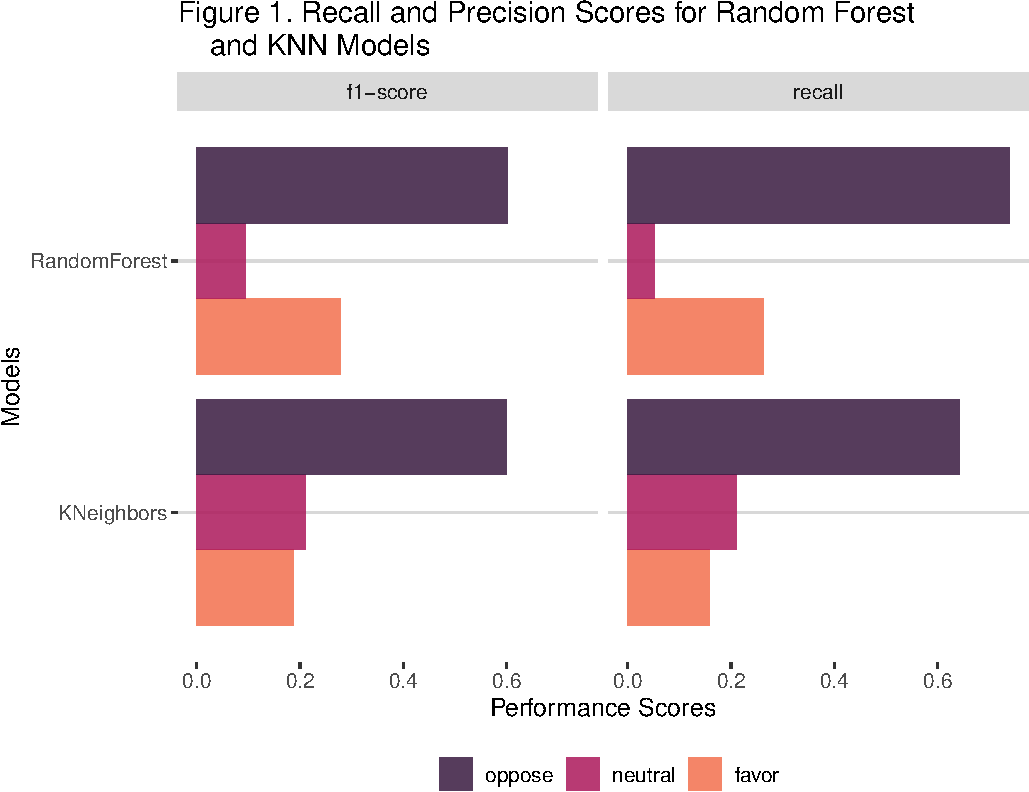
\includegraphics{assign_3_files/figure-pdf/unnamed-chunk-3-1.pdf}

The LLMs, showed poor performance in classifying the ``favor'' stance,
with very low f1-scores (llama .07: gemma .02) despite moderate recall
(llama .29: gemma .33), indicating low precision (see Figure 2). For the
``neutral'' class, both models showed modest results, with llama
achieving a slightly better F1-score (.23) compared to gemma (0.18),
although gemma had a higher recall (.50 vs .25), again suggesting lower
precision for gemma. Similar to the supervised models, both LLMs
performed best in classifying the ``oppose'' stance, with relatively
high and similar F1-scores (llama .67: gemma .70) and comparable recall
(llama .56: gemma .56), suggesting a better balance between precision
and recall for this category. Both models correctly identify 67 to 70
percent of all the actual Reddit comments expressing opposition.
Overall, both LLMs struggled with the ``favor'' and ``neutral'' classes
but demonstrated a stronger ability to identify opposing comments.\\

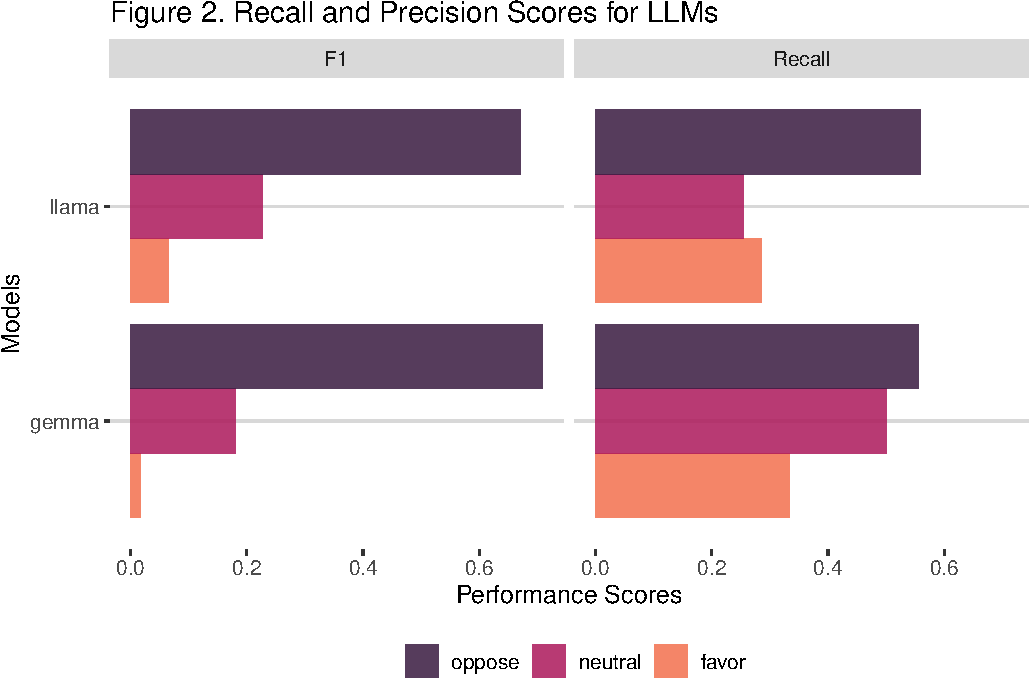
\includegraphics{assign_3_files/figure-pdf/unnamed-chunk-5-1.pdf}

Gemma and llama demonstrated only fair agreement in stance
classification (Cohen's Kappa = .24). The contingency table, Table 2
below, reveals highest agreement for ``oppose'' (.80), indicating some
consistency in identifying a strong negative stance. However, agreement
was substantially lower for ``neutral'' (.03) and ``favor'' (.01),
highlighting divergent interpretations of more nuanced language.
Off-diagonal values further illustrate these discrepancies, suggesting
fundamental differences in how the models process ambiguous cues and
establish classification boundaries, particularly for less extreme
stances.

\begin{longtable}[]{@{}lrrr@{}}
\caption{Aggreement between LLMs, Cohens Kappa, 0.24}\tabularnewline
\toprule\noalign{}
& favor & neutral & oppose \\
\midrule\noalign{}
\endfirsthead
\toprule\noalign{}
& favor & neutral & oppose \\
\midrule\noalign{}
\endhead
\bottomrule\noalign{}
\endlastfoot
favor & 3 & 1 & 10 \\
neutral & 0 & 10 & 49 \\
oppose & 0 & 5 & 317 \\
\end{longtable}

\section{Conclusion}\label{conclusion}

We explored public sentiment on Reddit regarding the DOGE federal
workforce reduction using supervised learning (KNN, Random Forest) and
unsupervised LLMs ( gemma 3.12b and Llama 3.2 3B) for stance
classification. Our supervised learning models achieved moderate success
in this classification task, with the strongest performance in
identifying opposing viewpoints, which were also the most prevalent in
our labeled data. Moreover, both models struggled with the ``favor'' and
``neutral'' stances, suggesting limitations in our initial features to
capture these nuances. Our unsupervised learning models also showed the
best ability to classify ``oppose'' comments, yet exhibited significant
challenges with the ``favor'' and ``neutral'' categories, particularly
demonstrating low precision.

This study had limitations such as the small size of our labelled
dataset of 400 Reddit, imbalance in the stance categories, and few
features in the supervised approach. The zero-shot capabilities of the
LLMs are suitable for topic exploration but may require fine-tuning for
optimal performance on this specific domain, particularly with nuance
language used in ``favor'' comments. Future research should continue to
understand federal worker perceptions and improve stance classification
by expanding labeled dataset and incorporate more contextual text rather
than single comment text. Fine tuning LLMs on a larger corpus with
relevant comments could render more accuracy in the classification task.




\end{document}
